\documentclass[aspectratio=169]{beamer}
\setbeamertemplate{navigation symbols}{}
\usepackage{color,amsmath,comment, subfigure}
\usepackage{booktabs}
\usepackage{url}

%\setbeameroption{show notes}

%%%%%%%%%%%%%%%%%%%%%%%%%%
\title[]{Lecture 3: More on the small world problem\\and some history}
\author[]{Sociology 204: Social Networks, Spring 2021}
\institute[]{Matthew J. Salganik}
\date[]{
1/3: Electronic small world experiment

\vfill

\begin{flushleft}
\vspace{0.7in}

\includegraphics[width=0.05\textwidth]{figures/cc.png}
\end{flushleft}
}

\begin{document}
%%%%%%%%%%%%%%%%%%%%%%%%%%%
\frame{\titlepage}
%%%%%%%%%%%%%%%%%%%%%%%%%%%
\begin{frame}

{\LARGE POP QUIZ}
\pause
{\LARGE FOR CANDY}

\pause
What was the chain completion rate for Dodds, Muhamad, and Watts?

\end{frame}
%%%%%%%%%%%%%%%%%%%%%%%%
\begin{frame}

Let's think back to 1967 . . . . 

\end{frame}
%%%%%%%%%%%%%%%%%%%%%%%%%%%
\begin{frame}

\begin{center}
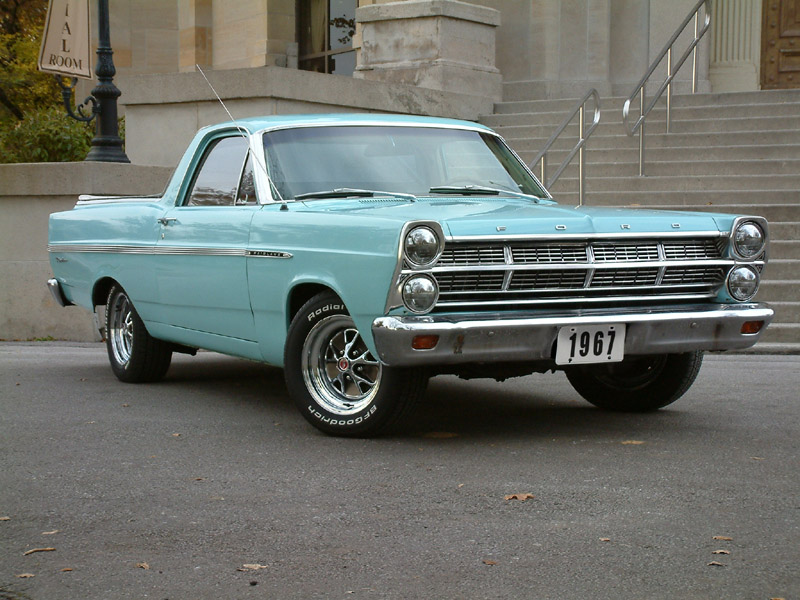
\includegraphics[height=0.8\textheight]{figures/1967_Ford_Fairlane_Ranchero.jpg}
\end{center}

\vfill
\tiny{\url{http://upload.wikimedia.org/wikipedia/commons/f/f5/1967_Ford_Fairlane_Ranchero.jpg}}

\end{frame}
%%%%%%%%%%%%%%%%%%%%%%%%%%%
\begin{frame}

\begin{center}
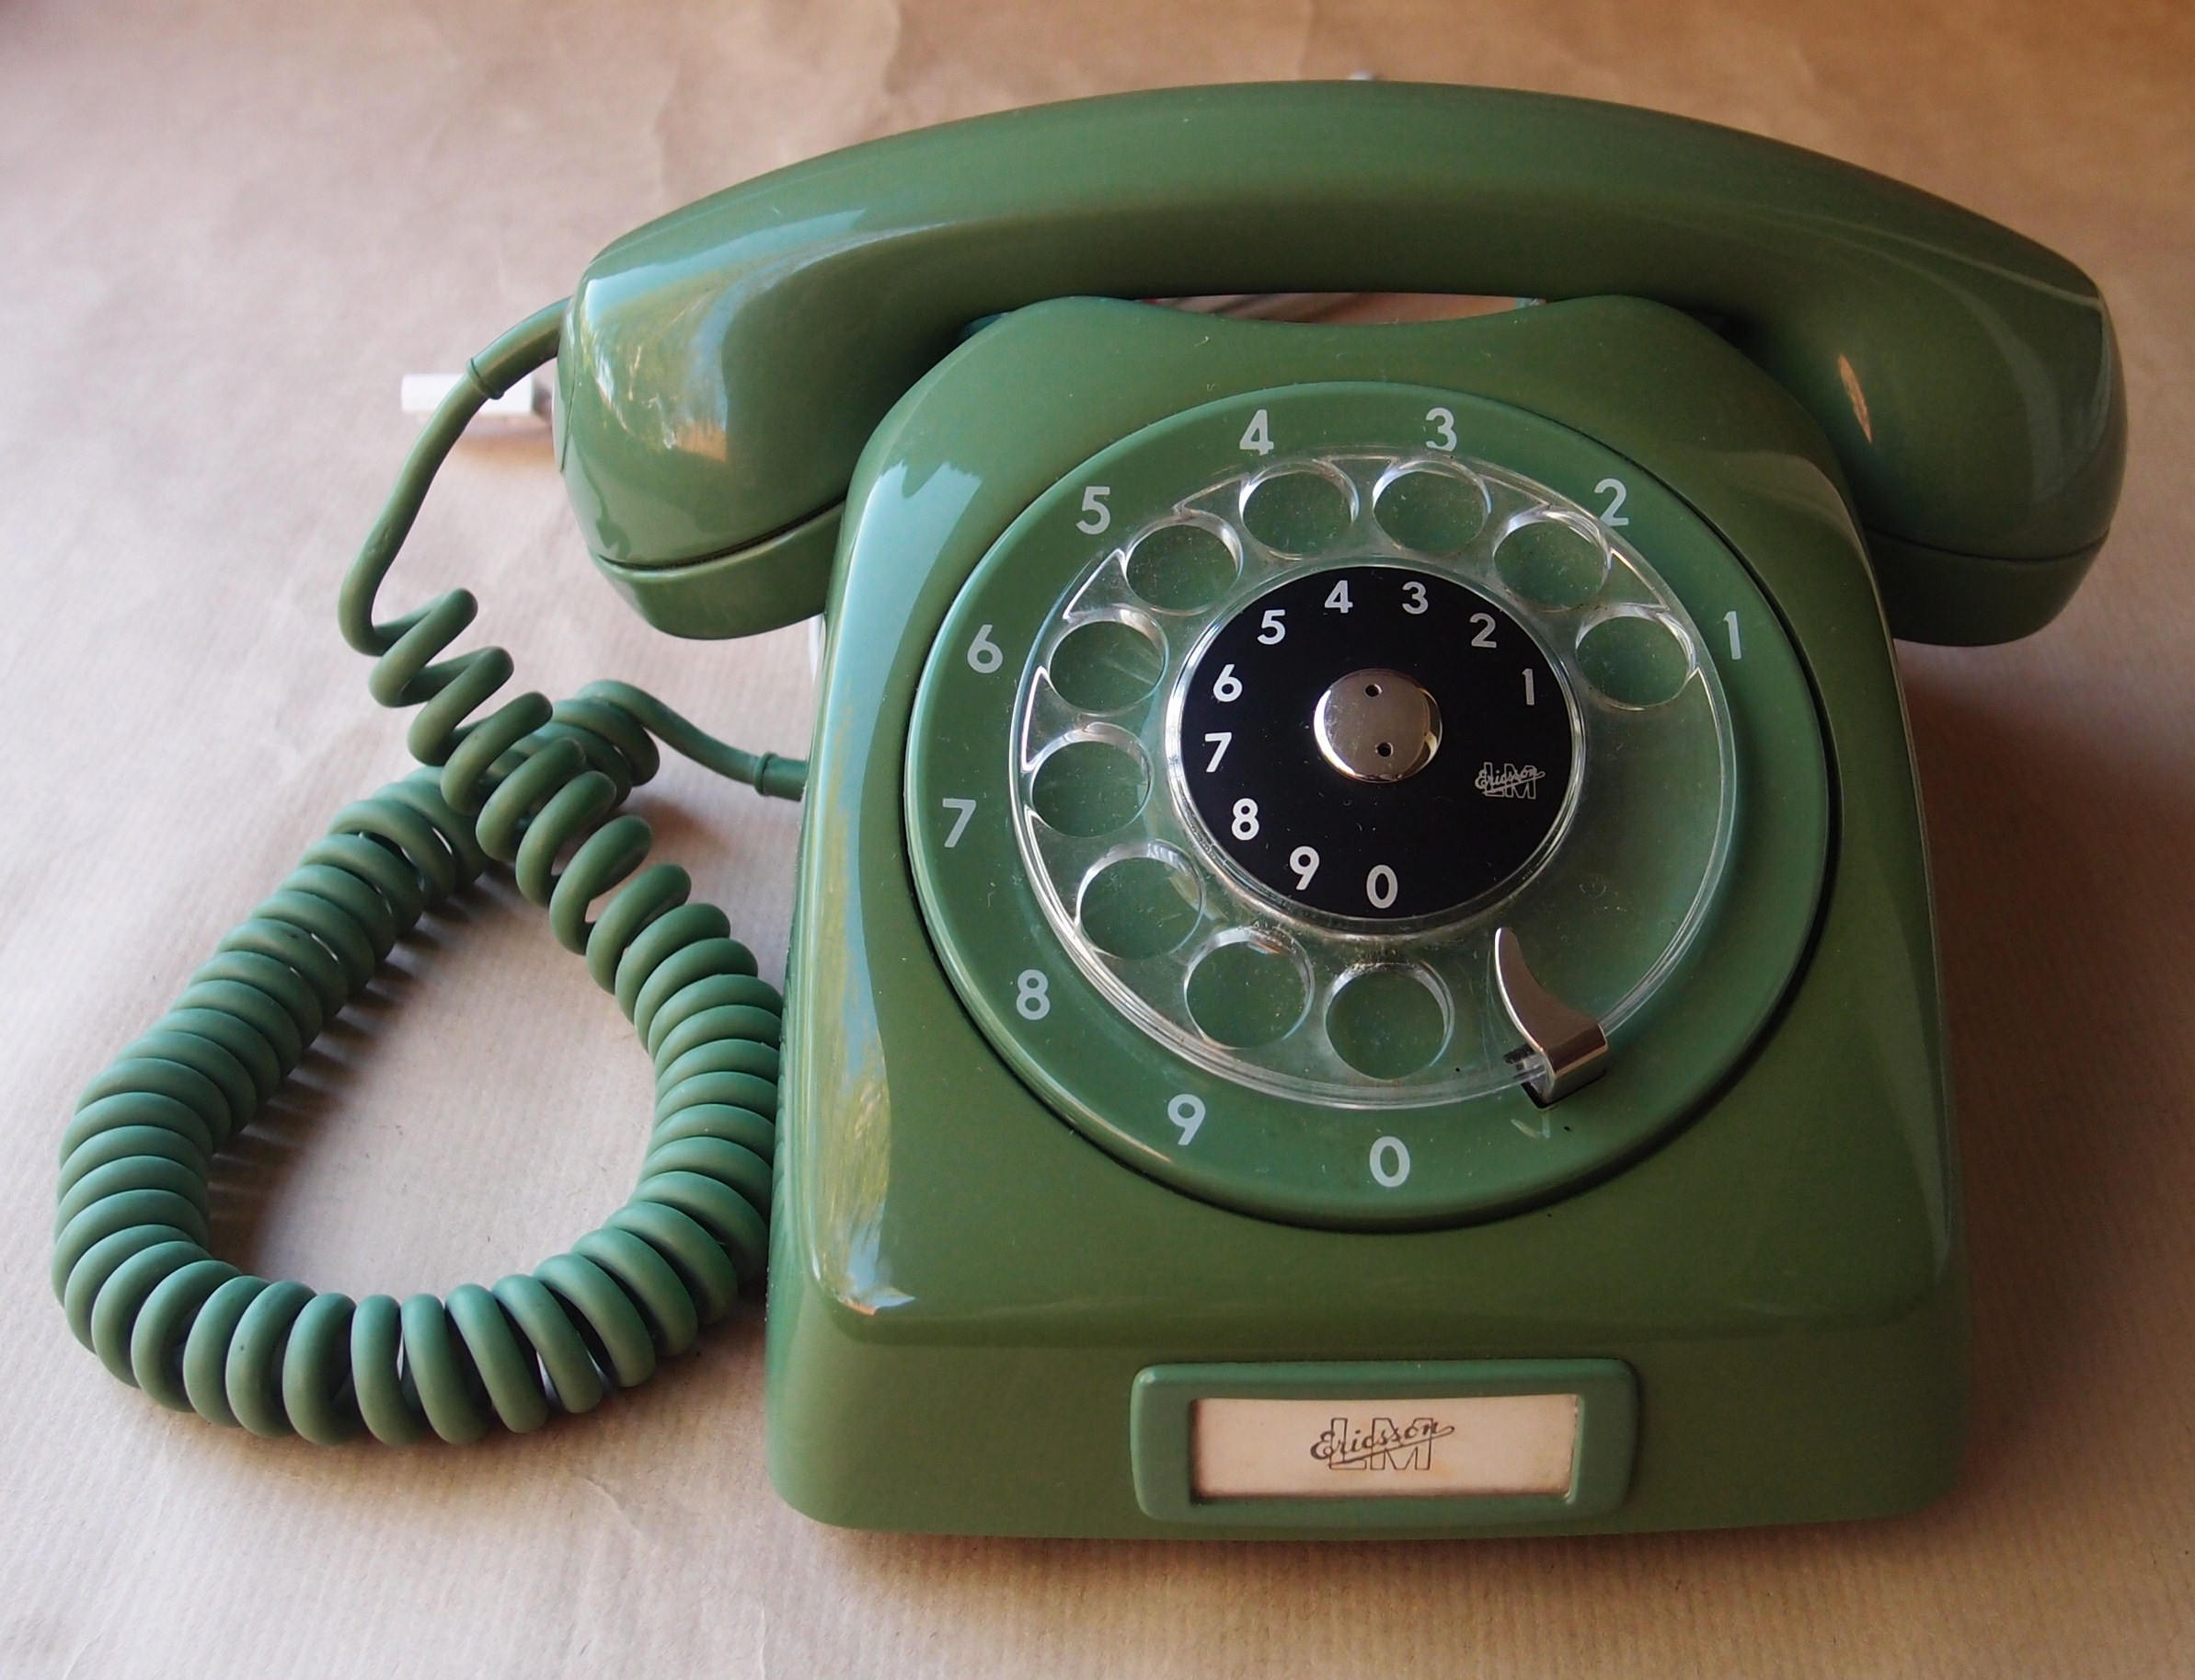
\includegraphics[height=0.8\textheight]{figures/Ericsson_Dialog_in_green}
\end{center}

\vfill
\tiny{\url{http://commons.wikimedia.org/wiki/File:Ericsson_Dialog_in_green.JPG}}

\end{frame}
%%%%%%%%%%%%%%%%%%%%%%%%%%%
\begin{frame}

\begin{center}
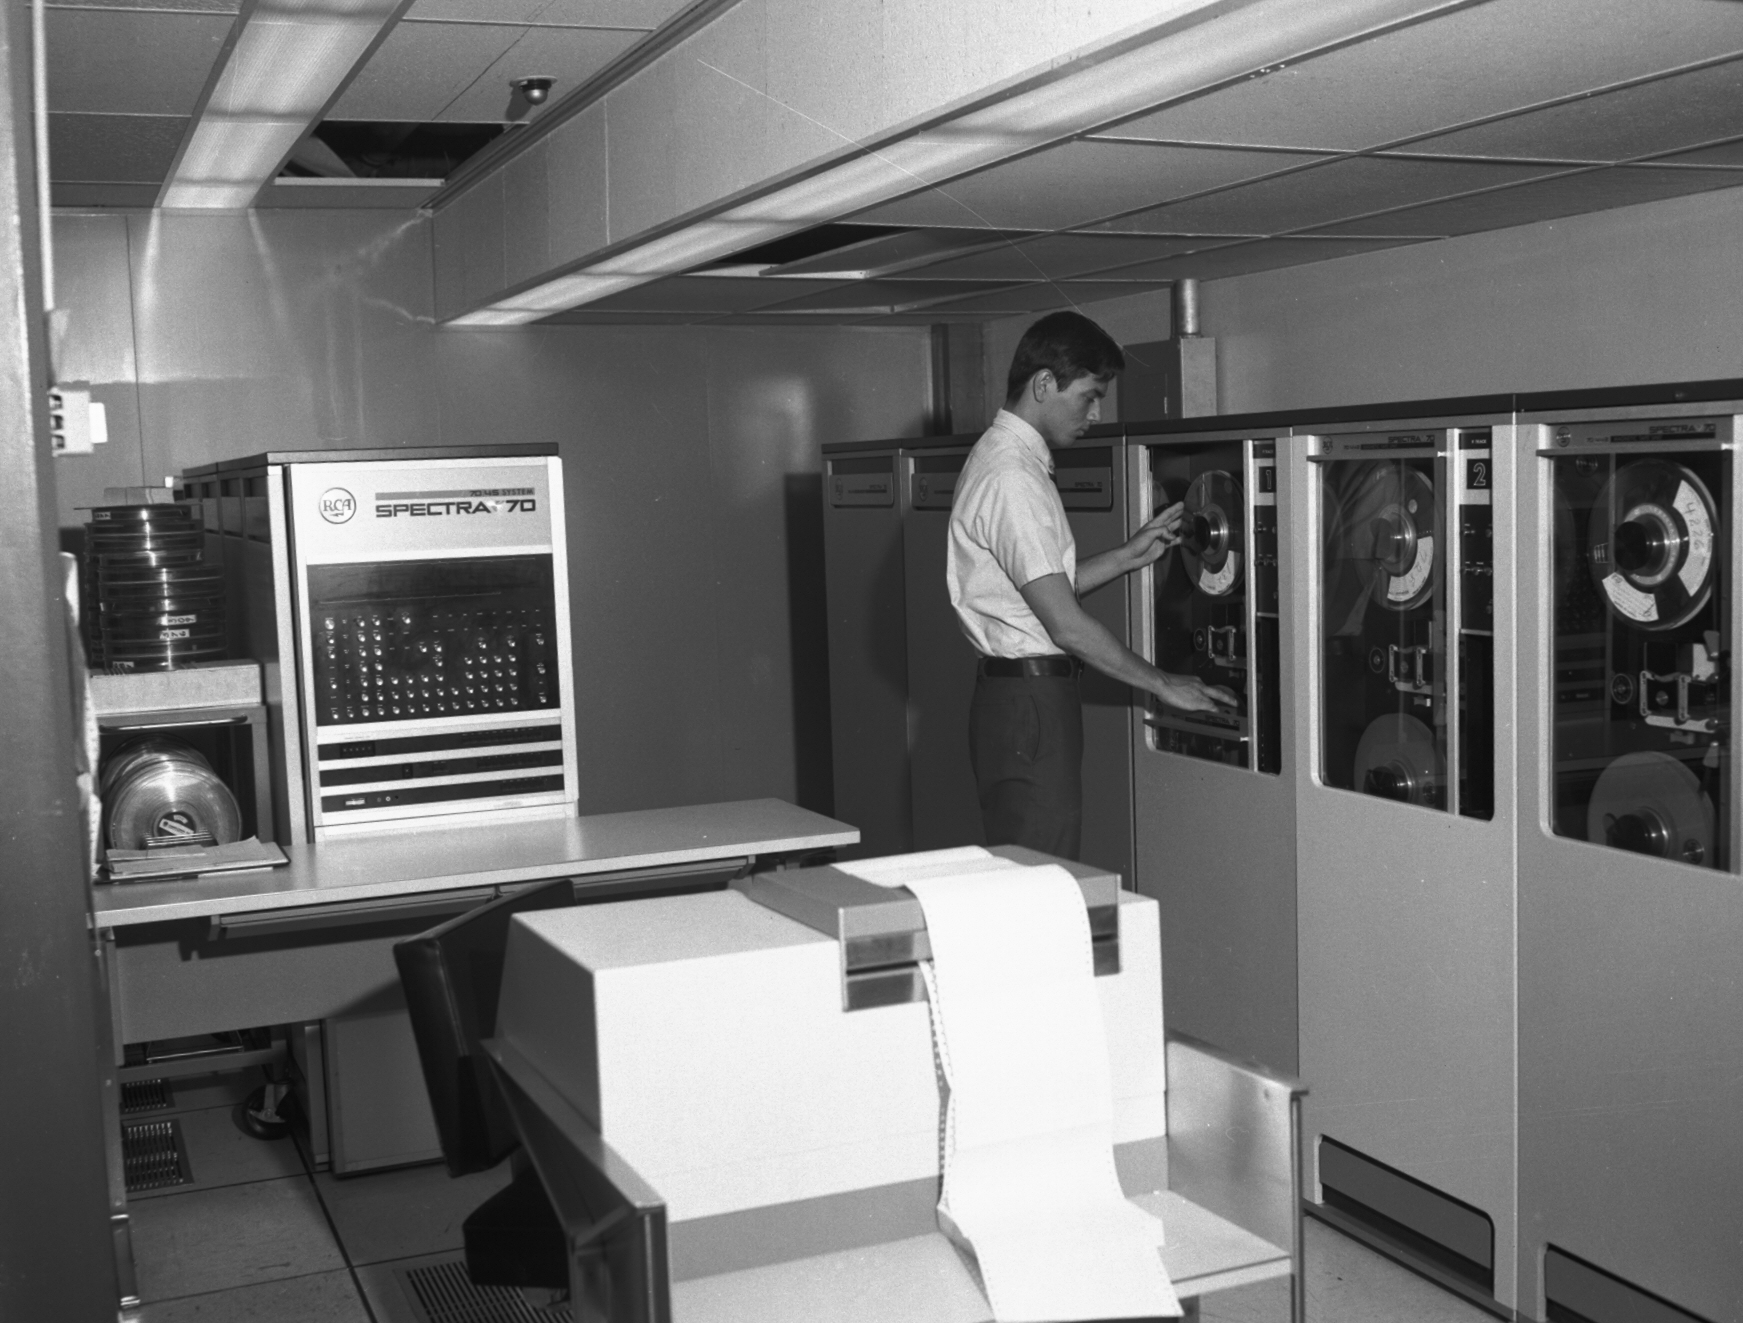
\includegraphics[height=0.8\textheight]{figures/Computer_in_County_of_Orange_offices,_1967}
\end{center}

\vfill
\tiny{\url{http://commons.wikimedia.org/wiki/File:Computer_in_County_of_Orange_offices,_1967.jpg}}

\end{frame}
%%%%%%%%%%%%%%%%%%%%%%%%%%%
\begin{frame}

Story $\rightarrow$ problem statement

\end{frame}
%%%%%%%%%%%%%%%%%%%%%%%%%%%
\begin{frame}

Given two individuals selected randomly from the population, what is the probability that the minimum number of intermediaries required to link them is 0,1,2,...k?

\end{frame}
%%%%%%%%%%%%%%%%%%%%%%%%%%%
\begin{frame}

\begin{center}
\begin{columns}
\begin{column}{0.4\textwidth}
Empirical approach\\(Harvard approach)
\end{column}
\begin{column}{0.2\textwidth}
vs.
\end{column}
\begin{column}{0.4\textwidth}
Modeling approach\\(MIT approach)
\end{column}
\end{columns}
\end{center}

\pause
\vfill
Today
\begin{itemize}
\item see how Dodds, Muhamad, and Watts tried to improve the empirical approach
\item learn some background so that we can understand a modeling approach
\end{itemize}

\end{frame}
%%%%%%%%%%%%%%%%%%%%%%%%%%%
\begin{frame}

``I read somewhere that everybody on the planet is separated by only six other people.  Six degrees of separation.  Between us and everybody else on this planet.  The president of the United States.  A gondolier in Venice . . . It's not just the big names.  It's anyone.  A native in the rain forest.  A Tierra del Fuegan.  An Eskimo.  I am bound to everyone on this planet by a trail of six people.  It's a profound thought . . . ''\\
Ouisa in \textit{Six Degrees of Separation} by John Guare (1990)

\note{
Dodds et al read all the paper and they were probably also influenced by Guare
Milgram talks about 200 million americas
Guare scales it up to the world
Scientists try to test this literary idea
}

\end{frame}
%%%%%%%%%%%%%%%%%%%%%%%%%%%%%
\begin{frame}

{\Large
\begin{center}
Analog vs Digital
\end{center}}

\end{frame}
%%%%%%%%%%%%%%%%%%%%%%%%%%%
\begin{frame}

Digital enables:
\begin{itemize}
\item zero-marginal cost data
\end{itemize}

\end{frame}
%%%%%%%%%%%%%%%%%%%%%%%%%%%%
\begin{frame}

\begin{center}
\includegraphics<1>[height = 0.95\textheight]{figures/zero_variable_cost_1}
\includegraphics<2>[height = 0.95\textheight]{figures/zero_variable_cost_2}
\end{center}

\note{
talk about scaling in each study
}

\end{frame}
%%%%%%%%%%%%%%%%%%%%%%%%%%%%
\begin{frame}

Digital enables:
\begin{itemize}
\item zero-marginal cost data
\item 100x'ing the number of participants
\pause
\item global scale
\end{itemize}

\pause
\vfill For more: Salganik (2018) \textit{Bit by Bit: Social Research in the Digital Age}: \url{http://www.bitbybitbook.com}

\note{
Global scale: imagine all the stamps and logistics
}

\end{frame}
%%%%%%%%%%%%%%%%%%%%%%%%%%%%
\begin{frame}

\begin{itemize}
\item What was the limiting factor for Travers and Milgram?
\item What was the limiting factor for Dodds, Muhamad, and Watts?
\end{itemize}

\end{frame}
%%%%%%%%%%%%%%%%%%%%%%%%%%%
\begin{frame}

24,163 chains started toward 18 targets all over the world.  The first time ever we have an experiment like this on a global scale.  What did they find?  

\note{The biggest study ever, years of coding in the basement, what did they find?}

\end{frame}
%%%%%%%%%%%%%%%%%%%%%%%%%%%%
\begin{frame}

\begin{center}
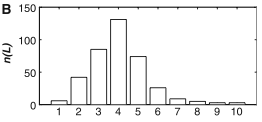
\includegraphics[width = 0.95\textwidth]{figures/dodds_experimental_2003_fig2b}
\end{center}

\vfill
$L =$ chain length (number of edges)

\note{Mean of 4 intermediaries, but remember this data is misleading because of attrition.  Think back to the coin flipping experiment.}

\end{frame}
%%%%%%%%%%%%%%%%%%%%%%%%%%%
\begin{frame}

\begin{center}
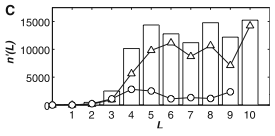
\includegraphics[width = 0.95\textwidth]{figures/dodds_experimental_2003_fig2c}
\end{center}

\vfill
Median of 5 (same country) to 7 (different country) intermediaries

\note{Median of 5 - 7 intermediaries}

\end{frame}
%%%%%%%%%%%%%%%%%%%%%%%%%%%
\begin{frame}

How did people decide who to pass the message to?\\

Location and occupation accounted for about half of all choices

\end{frame}
%%%%%%%%%%%%%%%%%%%%%%%%%%%
\begin{frame}

What was the chain completion rate for Dodds, Muhamad, and Watts?

\end{frame}
%%%%%%%%%%%%%%%%%%%%%%%%%%%
\begin{frame}

\begin{center}
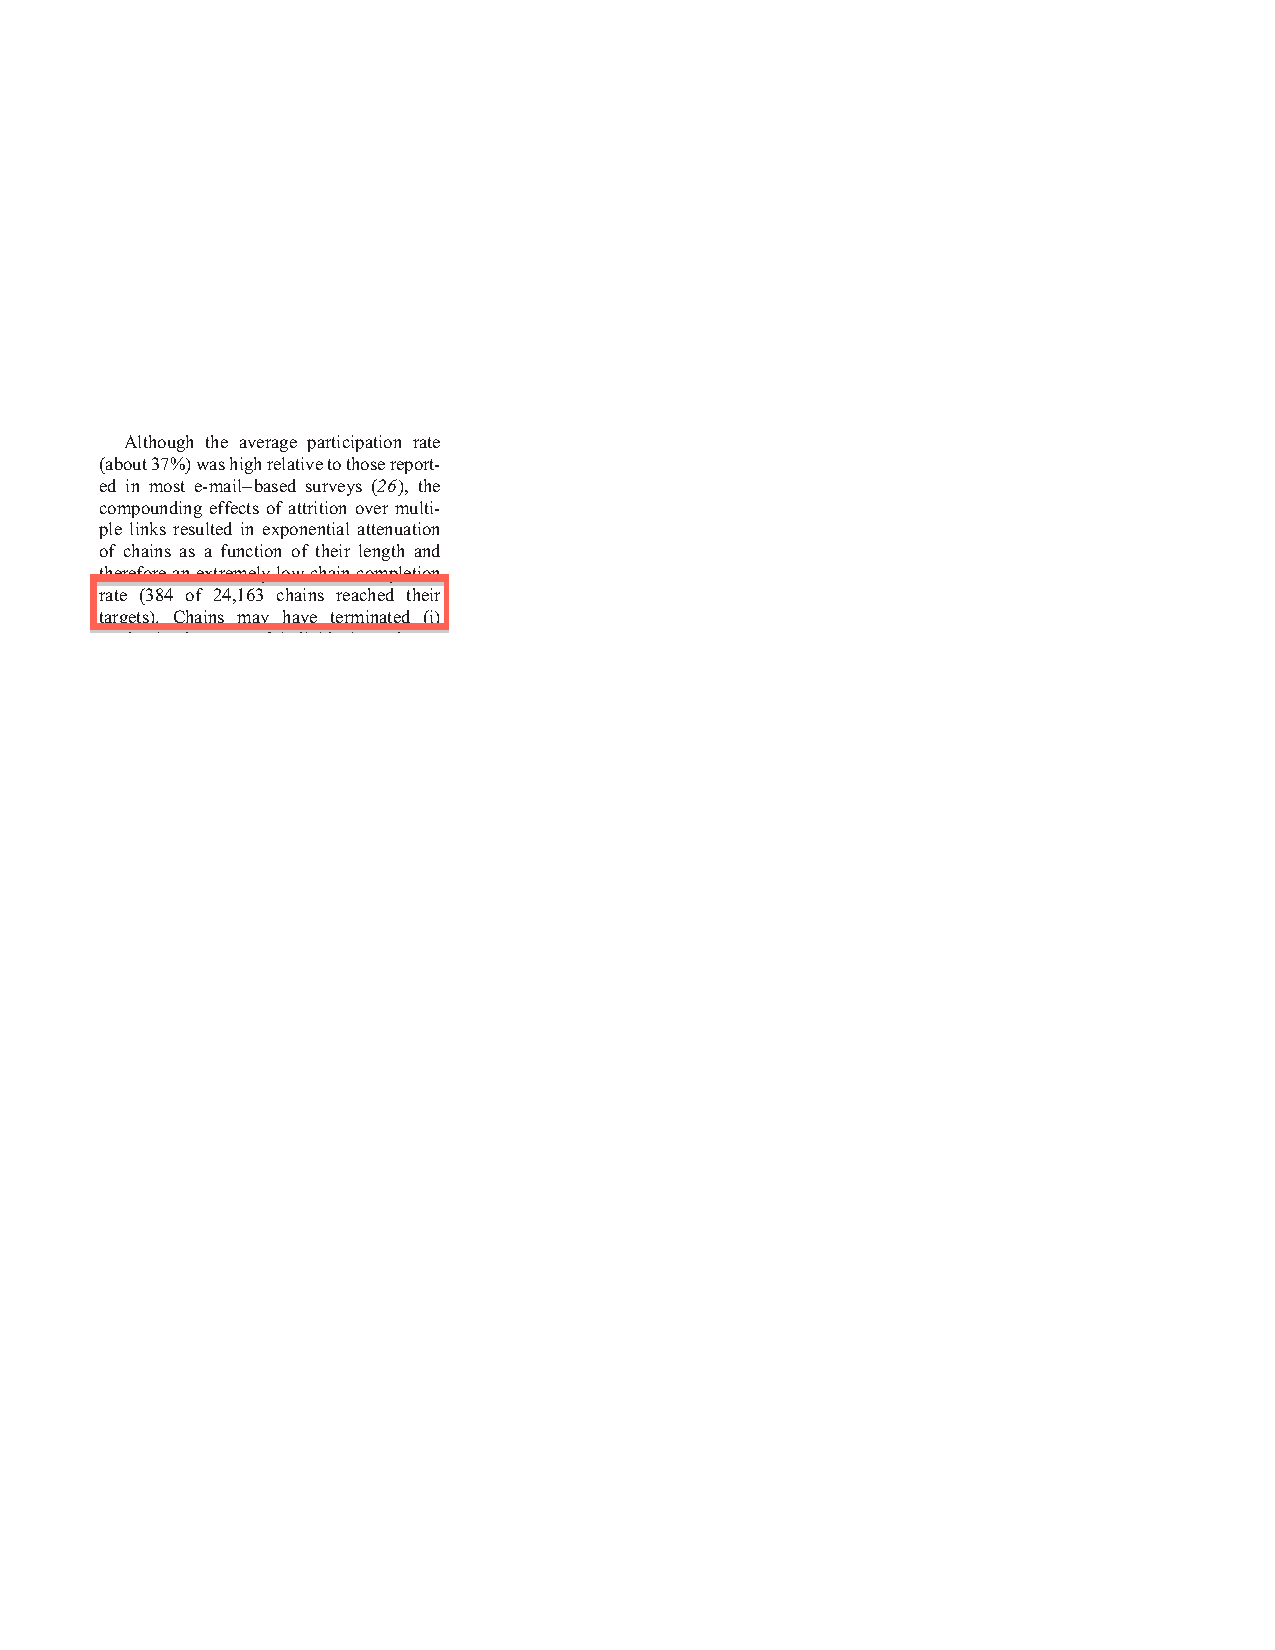
\includegraphics[width=0.9\textwidth]{figures/dodds_experimental_2003_completion}
\end{center}
\begin{center}
$\frac{384}{24,163}= \textcolor{blue}{1.6\%}$
\end{center}

\note{24,163 initiated only 384 completed (that's 1.6\%)  98.4\% didn't complete.  Notice that the number 1.6\% is not in the paper anywhere, 98.4\% certainly not.  

Why is this important. The actual number is not important, but this is an important lesson in how to be an alert reader.   See who gets candy.

Like a magician: look over here and not over here
}

\end{frame}
%%%%%%%%%%%%%%%%%%%%%%%%%%%
\begin{frame}

\begin{center}
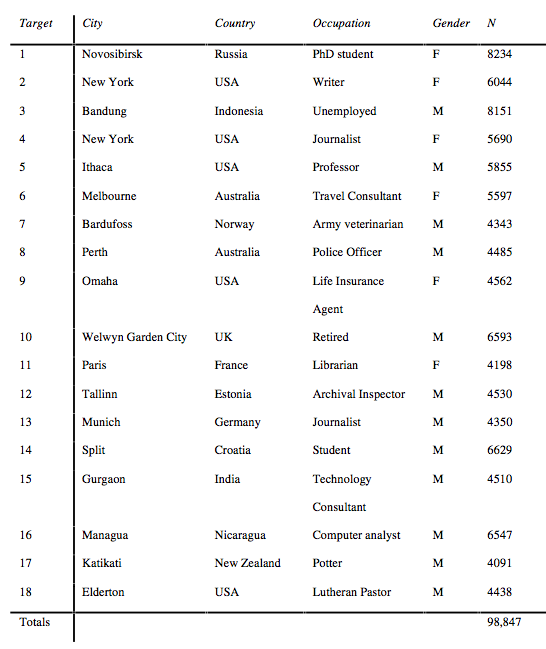
\includegraphics[height = 0.95\textheight]{figures/dodds_experimental_2003_tabS1_partial}
\end{center}

\note{
With Travers and Milgram there was one target, here 18.  What can we learn from that?
\begin{itemize}
\item Who had the lowest completion rate?
unemployed person in Indonesia.  He's probably Roby's friend.  Hard to find him because occupation can't be used for search.
student in Croatia.  Also, probably hard to find because of occupation is not a helpful dimension for search
\item Who had the highest completion rate?
Professor in Ithaca: Steve Strogatz and he's not that special (socially at least)
\end{itemize}
}

\end{frame}
%%%%%%%%%%%%%%%%%%%%%%%%%%%
\begin{frame}

\begin{center}
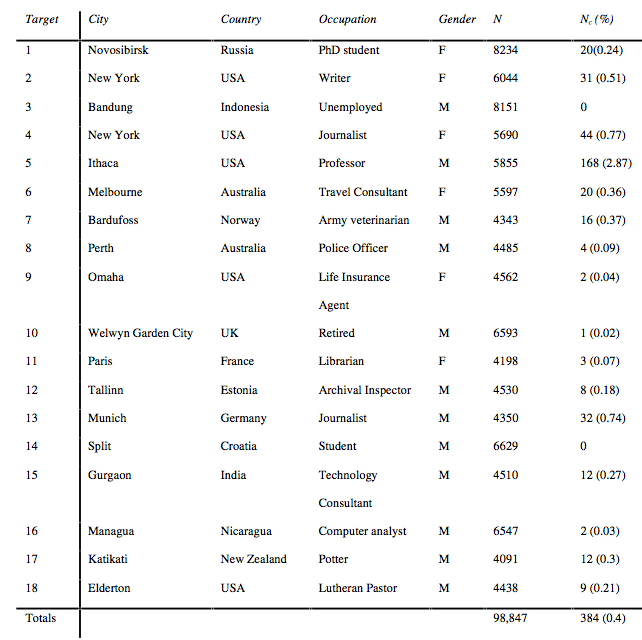
\includegraphics[height = 0.95\textheight]{figures/dodds_experimental_2003_tabS1_full}
\end{center}

\end{frame}
%%%%%%%%%%%%%%%%%%%%%%%%%%%
\begin{frame}

The largest empirical study of all time is mostly about connections to Steve Strogatz! (About 40\% of completed chains)

\note{

This is just hard to study empirically.  Just like certain astronomical measurements are hard to make, this measurement is hard to make.  Meta note: When you are reading the papers, make sure not read them individually, but think about how they link together.  It seems like short chains may exist, but it is hard to collect data on them.  Recall that Milgram began his experiments because theoretical approaches were not working.  Here we have run into a data wall and now will go back to theory.

}

\end{frame}
%%%%%%%%%%%%%%%%%%%%%%%%%%%
\begin{frame}

What's next?

\end{frame}
%%%%%%%%%%%%%%%%%%%%%%%%%%%
\begin{frame}

\begin{center}
\begin{columns}
\begin{column}{0.4\textwidth}
Empirical approach\\(Harvard approach)
\end{column}
\begin{column}{0.2\textwidth}
vs.
\end{column}
\begin{column}{0.4\textwidth}
Modeling approach\\(MIT approach)
\end{column}
\end{columns}
\end{center}

\end{frame}
%%%%%%%%%%%%%%%%%%%%%%%%%%%
\begin{frame}

\begin{center}
\begin{columns}
\begin{column}{0.4\textwidth}
Empirical approach\\(Harvard approach)
\end{column}
\begin{column}{0.2\textwidth}
vs.
\end{column}
\begin{column}{0.4\textwidth}
\textcolor{blue}{Modeling approach\\(MIT approach)}
\end{column}
\end{columns}
\end{center}

\end{frame}

\end{document}
